\maketitle
\tableofcontents
\newpage
\section{Theorie}
Gegenstand des Versuchs ist die Untersuchung von Strömungen mithilfe des
Impuls-Echo-Verfahrens der Ultraschalltechnik. Das Impuls-Echo-Verfahren beruht auf dem akustischen Dopplereffekt,
also der Frequenzveränderung einer Schallwelle bei einer Relativbewegung zwischen Quelle
und Sender. Benutzt wird dabei das als Ultraschall bezeichnete Frequenzband zwischen
\SI{20}{\kilo\hertz} und \SI{1}{\giga\hertz}. Unterschieden wird beim akustischen
Dopplereffekt zwischen zwei Fällen:
\begin{enumerate}
  \item \textbf{Bewegte Quelle - Ruhender Empfänger:}
  Bei Annäherung einer mit Geschwindigkeit $v$ bewegten Quelle misst der Beobachter eine um den
  Faktor $\left(1 - \frac{v}{c} \right)^{-1}$ erhöhte gesendete Frequenz $\nu_0$, bewegt sich
  die Quelle in die andere Richtung, so sinkt $\nu_0$ um den Faktor $\left(1 + \frac{v}{c} \right)^{-1}$.
  Zusammenfassend ist die gemessene Frequenz also durch
  \begin{equation}
    \label{eq:1}
    \nu_{\symup{kl/gr}} = \frac{\nu_0}{1 \mp \frac{v}{c}}
  \end{equation}
  gegeben.
  \item \textbf{Bewegter Empfänger - Ruhende Quelle:}
  In diesem Fall bewirkt eine Annäherung eine Verschiebung von $\nu_0$ um den Faktor
  $ \left(1+ \frac{v}{c} \right) $, im umgekehrten Fall tritt eine Verminderung um den
  $ \left(1- \frac{v}{c} \right) $, allgemein also:
  \begin{equation}
    \label{eq:2}
    \nu_{\symup{h/n}} = \nu_0 \left( 1 \pm \frac{v}{c} \right)
  \end{equation}
\end{enumerate}
In der Doppler-Sonographie findet nun der zweite Fall Anwendung um unter anderem
Strömungsgeschwindigkeiten zu bestimmen. Aus \eqref{eq:2} folgt eine Frequenzverschiebung von
\begin{equation}
  \label{eq:3}
  \symup{\Delta}\nu = \nu_0 \frac{v}{c} (\cos{\alpha} + \cos{\beta}),
\end{equation}
die Winkel $\alpha$ und $\beta$  sind dabei die zwischen dem Geschwindigkeitsvektor des
beobachteten Teilchens und dem Normalenvektor der einlaufenden bzw. der am Objekt reflektierten
auslaufenden Wellenfront eingeschlossenen Winkel. Beim Impuls-Echo-Verfahren sind
Sender und Empfänger in einem Gerät zusammengefasst, sodass $\alpha$ und $\beta$ gleich sind
und aus \eqref{eq:3}
\begin{equation}
  \label{eq:4}
  \symup{\Delta}\nu = 2 \nu_0 \frac{v}{c} \cos{\alpha}
\end{equation}
folgt. Das Verfahren ist in Abbildung \ref{abb:1} dargestellt.
\begin{figure}
  \centering
  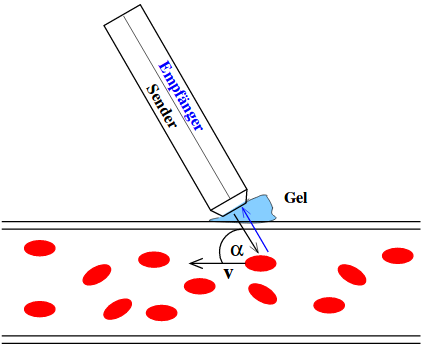
\includegraphics[scale=0.35]{blutbahn.png}
  \caption{Schematische Skizze der Doppler-Sonographie \cite{anleitung}.}
  \label{abb:1}
\end{figure}
Erzeugt werden kann Ultraschall unter Zuhilfenahme des piezo-elektrischen Effekts.
Ein piezoelektrischer Kristall, meist Quarze, wird durch ein sich periodisch änderndes elektrisches Feld
zu Schwingungen angeregt und strahlt dadurch Ultraschallwellen ab. Stimmt die anregende
Frequenz im Resonanzfall mit der Eigenfrequenz des Kristalls überein,
erreichen die abgestrahlten Ultraschallwellen hohe Amplituden und damit auch hohe Energiedichten.
Der piezo-elektrische Effekt an Kristallen kann im umgekehrten Fall zur Konstruktion
eines Empfängers genutzt werden. Einlaufende Schallwellen regen den Kristall dabei zu Schwingungen an.
\section{Durchführung}
\subsection{Versuchsaufbau}
\label{aufbau}
Der Versuchsaufbau besteht aus einem Flüssigkeitskreislauf, in dem eine Zentrifugalpumpe eine Strömung
erzeugt. Die Strömungsgeschwindigkeit lässt sich dabei stufenlos durch Veränderung
der Pumpleistung regeln. In den Kreislauf integriert sind gerade Rohrstücke
mit verschiedenen Durchmessern, auf die ein Dopplerprisma aus Acryl aufgesetzt wird,
dessen Oberseite drei vordefinierte Einstrahlwinkel $\theta$
(\SI{15}{\textdegree}, \SI{30}{\textdegree} und \SI{60}{\textdegree}) ermöglicht (siehe Abbildung \ref{abb:2}).
\begin{figure}
  \centering
  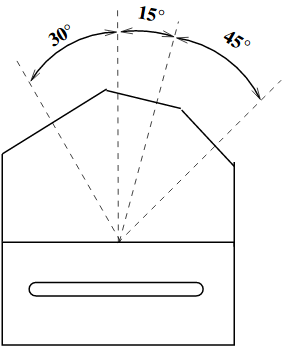
\includegraphics[scale=0.35]{DopplerPrisma.png}
  \caption{Skizze eines Dopplerprismas mit eingezeichneten Einstrahlwinkeln \cite{anleitung}.}
  \label{abb:2}
\end{figure}
Alle Kontaktflächen werden mit einem
Gel eingerieben, um die Übertragung der Ultraschallwellen zu optimieren.
Den Einstrahlwinkeln wird mit der Schallgeschwindigkeiten der Flüssigkeit ($c_\symup{L}$) und des Prismas
($c_\symup{P}$) durch das Brechungsgesetz ein Dopplerwinkel
\begin{equation}
  \label{eq:5}
  \alpha = \SI{90}{\textdegree} - \arcsin \left( \sin \theta \cdot \frac{c_\symup{L}}
  {c_\symup{P}} \right)
\end{equation}
zugeordnet. Genutzt wird eine Schallfrequenz $\nu_0$ von \SI{2}{\mega\hertz}. Die Messsonde
ist währenddessen über einen Ultraschall Doppler-Generator mit einem Computer verbunden, auf dem ein
Messprogramm installiert ist, welches das Auslesen der gemessenen Daten ermöglicht. Die
verwendete Flüssigkeit ist bezüglich ihrer akustischen Eigenschaften auf die
verwendeten Frequenz angepasst.
\subsection{Versuchsdurchführung}
In einem ersten Teil wird die Strömungsgeschwindigkeit in einem Rohrstück aus den
verschiedenen Einstrahlwinkeln des Doppler-Prismas bestimmt. Es werden für
fünf verschiedene Pumpleistungen aus allen drei Einstrahlwinkeln die Frequenzverschiebung
$\symup{\Delta}\nu$ gemessen. Daraus ergibt sich nach Formel \eqref{eq:4} mit Formel \eqref{eq:5}
die Strömungsgeschwindigkeit. Die jeweiligen Verhältnisse $\symup{\Delta}\nu / \cos \alpha$
werden dann in Abhängigkeit der Strömungsgeschwindigkeit in einem Diagramm aufgetragen.\\
\\
In einer zweiten Messreihe wird das Strömungsprofil in einem \num{3/8}-Zoll Rohr
(ca. \SI{10}{\milli\meter}) unter einem Einstrahlwinkel von \SI{15}{\textdegree} bestimmt.
Gemessen wird bei einer Pumpleistung von \SI{45} und \SI{70}{\percent}. Der Ultraschall
Doppler-Generator wird so eingestellt, dass er eine variable Messtiefe ermöglicht.
Die Einstellung am Generator ist dabei in \SI{0.5}{\micro\second}-Schritten möglich,
die Umrechnung in \si{\milli\metre} ist materialabhängig. Es wird der komplette
Rohrduchmesser durchfahren und in \SI{0.75}{\milli\metre}-Abständen sowohl Strömungsgeschwindigkeit als
auch Streuintensitätswert gemessen. Die beiden Datenreihen werden in Abhängigkeit der
Messtiefe in einem Diagramm aufgetragen.

\section{Auswertung}
Die im Folgenden ausgewerteten Versuchsteile wurden an einem Rohr mit einem Durchmesser
von $\SI{0.01}{\meter}$ durchgeführt.

\subsection{Bestimmung der Strömungsgeschwindigkeit für die Dopplerwinkel.}
Um die Strömungsgeschwindigkeit zu bestimmmen, wird \eqref{eq:4}
umgeformt zu
\begin{equation}
    v = \frac{\symup{\Delta} \nu \cdot c}{2 \, \nu_0 \, \symup{cos} \, \alpha} \, .
    \label{eqn:6}
\end{equation}
Mit \eqref{eq:5} folgt für die Dopplerwinkel $\alpha$ aus \eqref{eqn:6}
\begin{table}
  \centering
  \begin{tabular}{c c}
    \toprule
    $\theta$ & $\alpha$ \\
    \midrule
    15° & 80.06° \\
    30° & 70.53° \\
    60° & 54.74° \\
    \bottomrule
  \end{tabular}
  \caption{Dopplerwinkel $\alpha$ zu den vordefinierten Einfallswinkeln $\theta$.}
  \label{tab:1}
\end{table}
mit $c_L = \SI{1800}{\meter\per\second}$ und $c_P = \SI{2700}{\meter\per\second}$.
Damit folgen die Ergebnisse für die drei Dopplerwinkel mit $\nu_0 = \SI{2}{\mega\hertz}$
und $c = \SI{1800}{\meter\per\second}$ mit dem jeweils passendem Diagramm.

\begin{figure}
  \begin{subfigure}{0.6\textwidth}
    \centering
      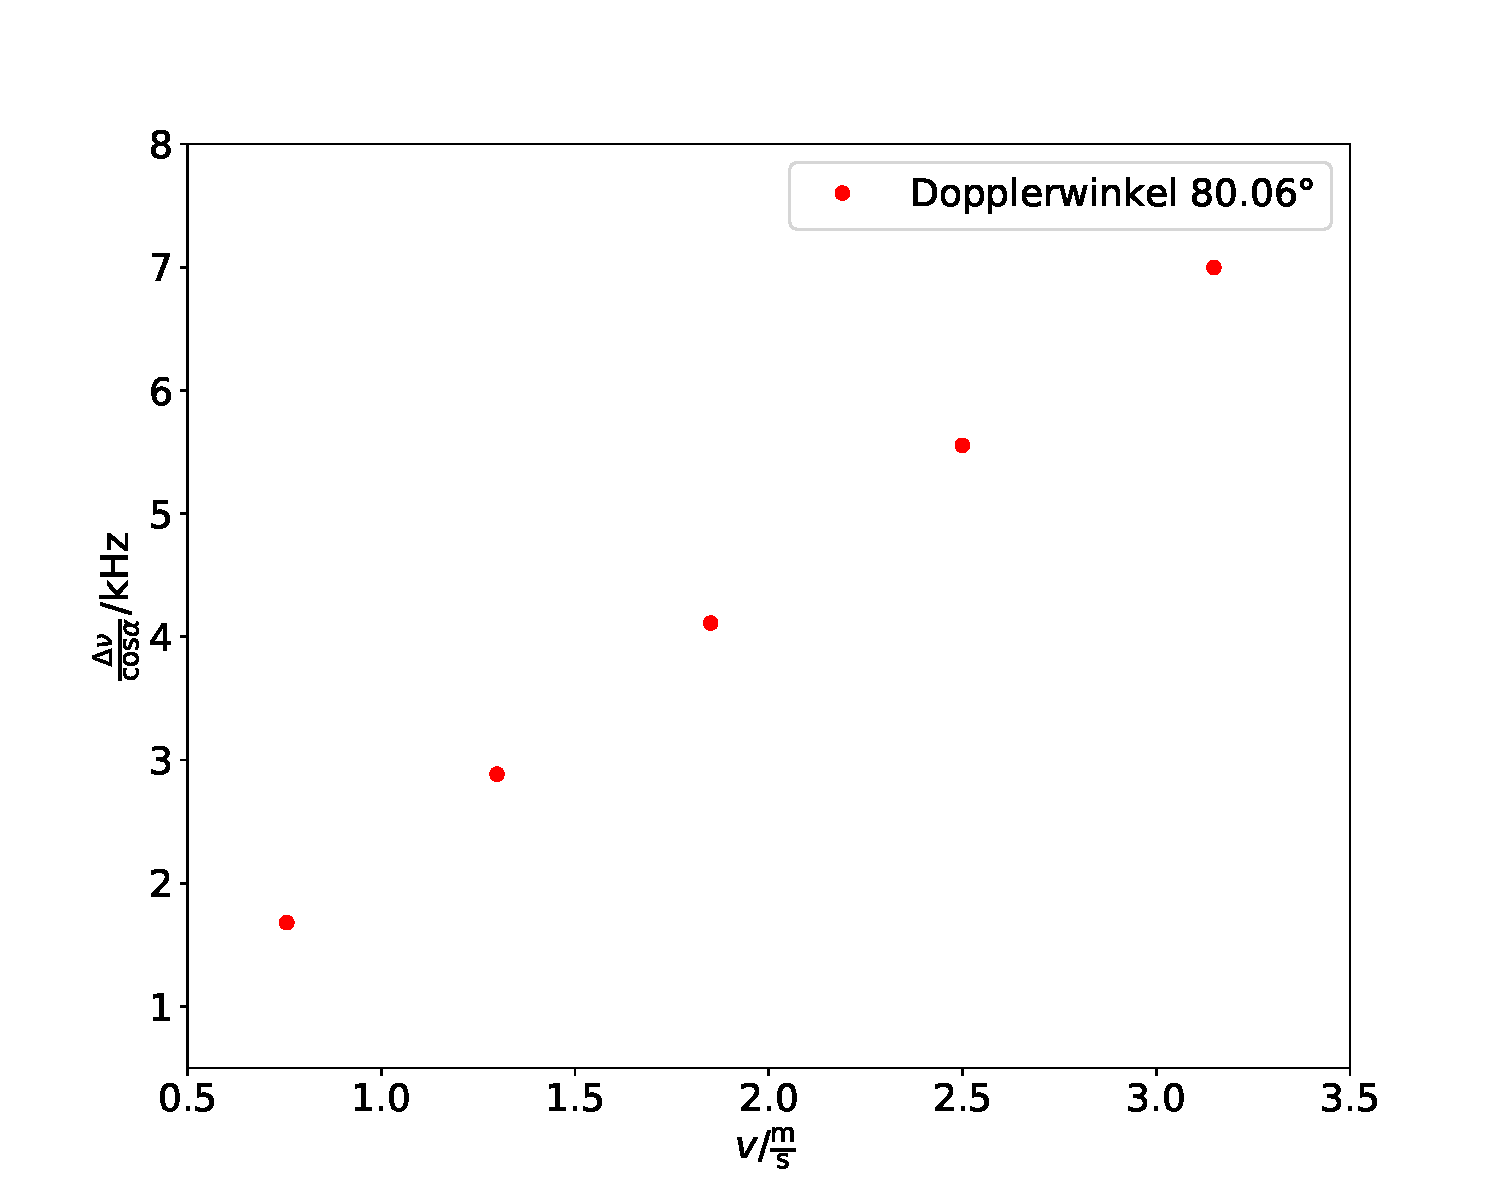
\includegraphics[width=\textwidth]{a15.pdf}
      \caption{Die Frequenzverschiebung geteilt durch den cos des Dopplerwinkels 80.06° aufgetragen gegen die Geschwindigkeit.}
      \label{fig:1}
      \qquad
  \end{subfigure}
  \begin{subtable}{0.4\textwidth}
    \centering
    \begin{tabular}{c c c}
      \toprule
      Pumpleistung / $\%$ & $\symup{\Delta} \nu$ / $\si{\hertz}$ & $v$ / \si{\meter\per\second} \\
      \midrule
      30 & -85 & 0.76 \\
      40 & -146 & 1.30 \\
      50 & -208 & 1.85 \\
      60 & -281 & 2.50 \\
      70 & -354 & 3.15 \\
      \bottomrule
    \end{tabular}
    \caption{Die Pumpleistung, die Frequenzverschiebung (aus den Messungen) und die Geschwindigkeit aus \eqref{eqn:6} berechnet für einen Einfallswinkel von 15°.}
    \label{tab:2}
    \qquad
  \end{subtable}
  \caption{Ergebnisse aus Aufgabenteil für den Dopplerwinkel 80.06°.}
\end{figure}

  \begin{figure}
      \begin{subfigure}{0.6\textwidth}
      \centering
        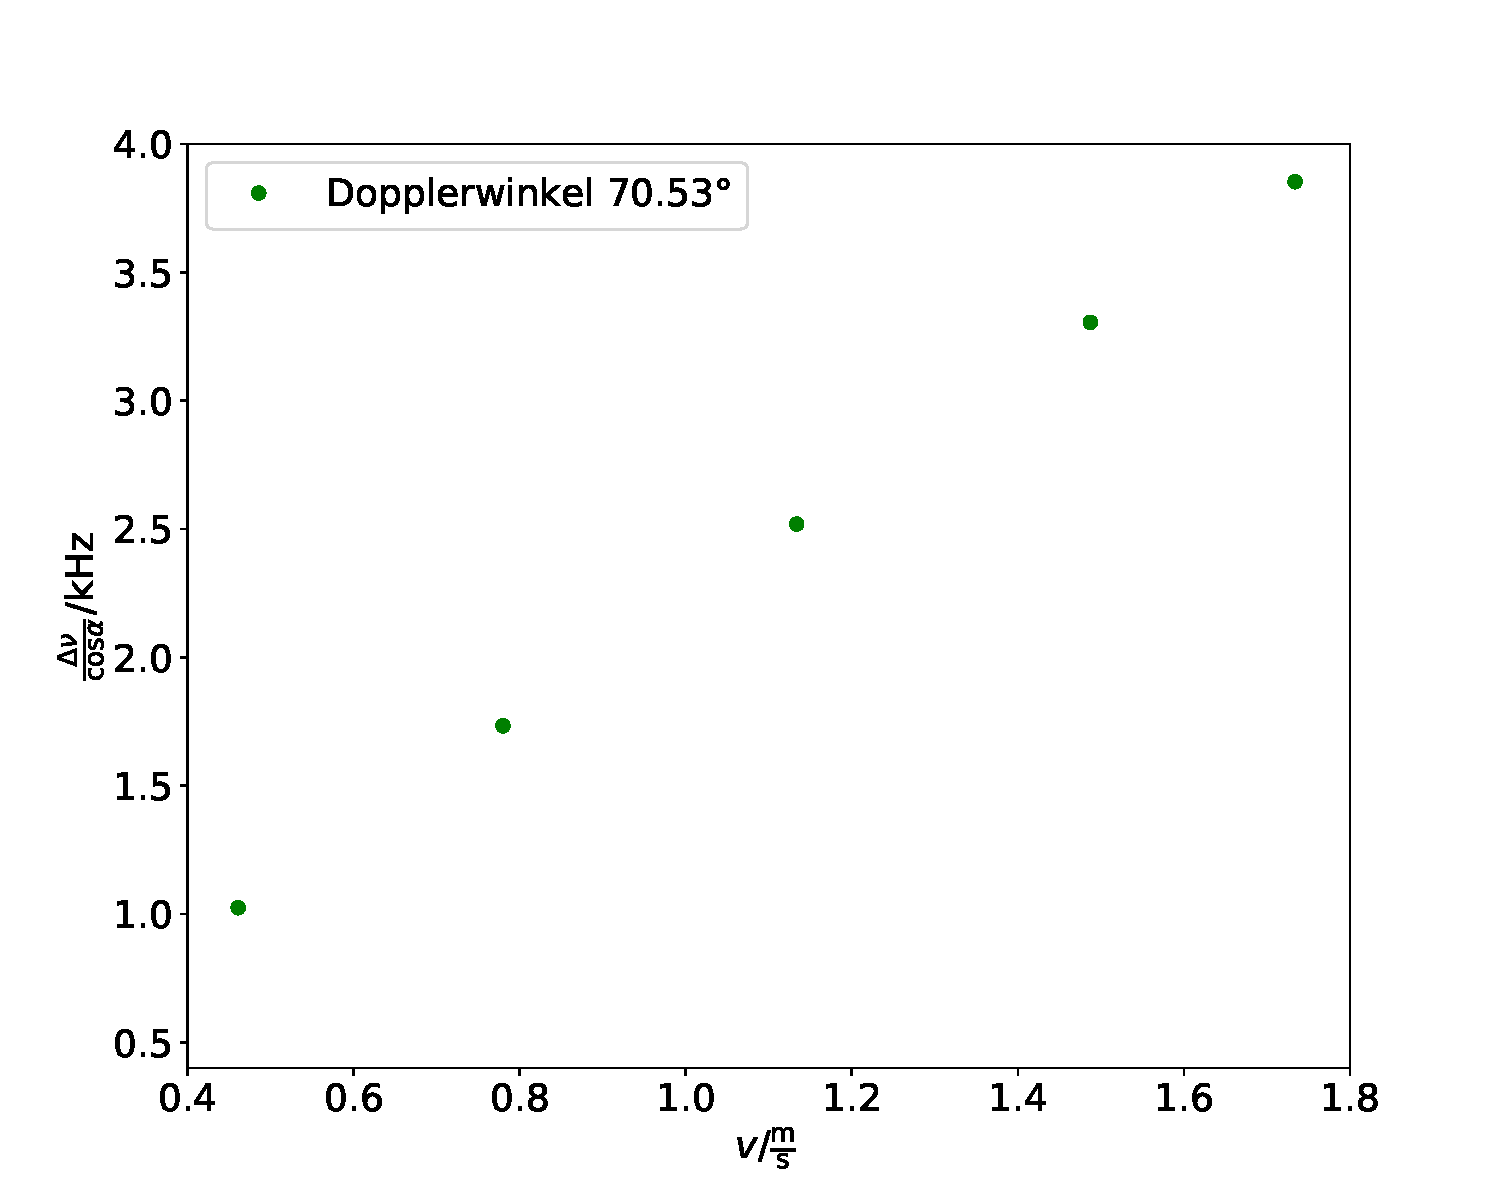
\includegraphics[width=\textwidth]{a30.pdf}
        \caption{Die Frequenzverschiebung geteilt durch den cos des Dopplerwinkels 70.53° aufgetragen gegen die Geschwindigkeit.}
        \label{fig:2}
        \qquad
    \end{subfigure}
    \begin{subtable}{0.4\textwidth}
      \centering
      \begin{tabular}{c c c}
        \toprule
        Pumpleistung / $\%$ & $\symup{\Delta} \nu$ / $\si{\hertz}$ & $v$ / \si{\meter\per\second} \\
        \midrule
        30 & 159 &  0.46 \\
        40 & 269 &  0.78 \\
        50 & 391 & 1.13  \\
        60 & 513 & 1.49  \\
        70 & 598 & 1.73 \\
        \bottomrule
      \end{tabular}
      \caption{Die Pumpleistung, die Frequenzverschiebung (aus den Messungen) und die Geschwindigkeit aus \eqref{eqn:6} berechnet für einen Einfallswinkel von 30°.}
      \label{tab:3}
      \qquad
    \end{subtable}
    \caption{Ergebnisse aus Aufgabenteil 1 für den Dopplerwinkel 70.53°.}
  \end{figure}
    \begin{figure}
      \begin{subfigure}{0.6\textwidth}
        \centering
          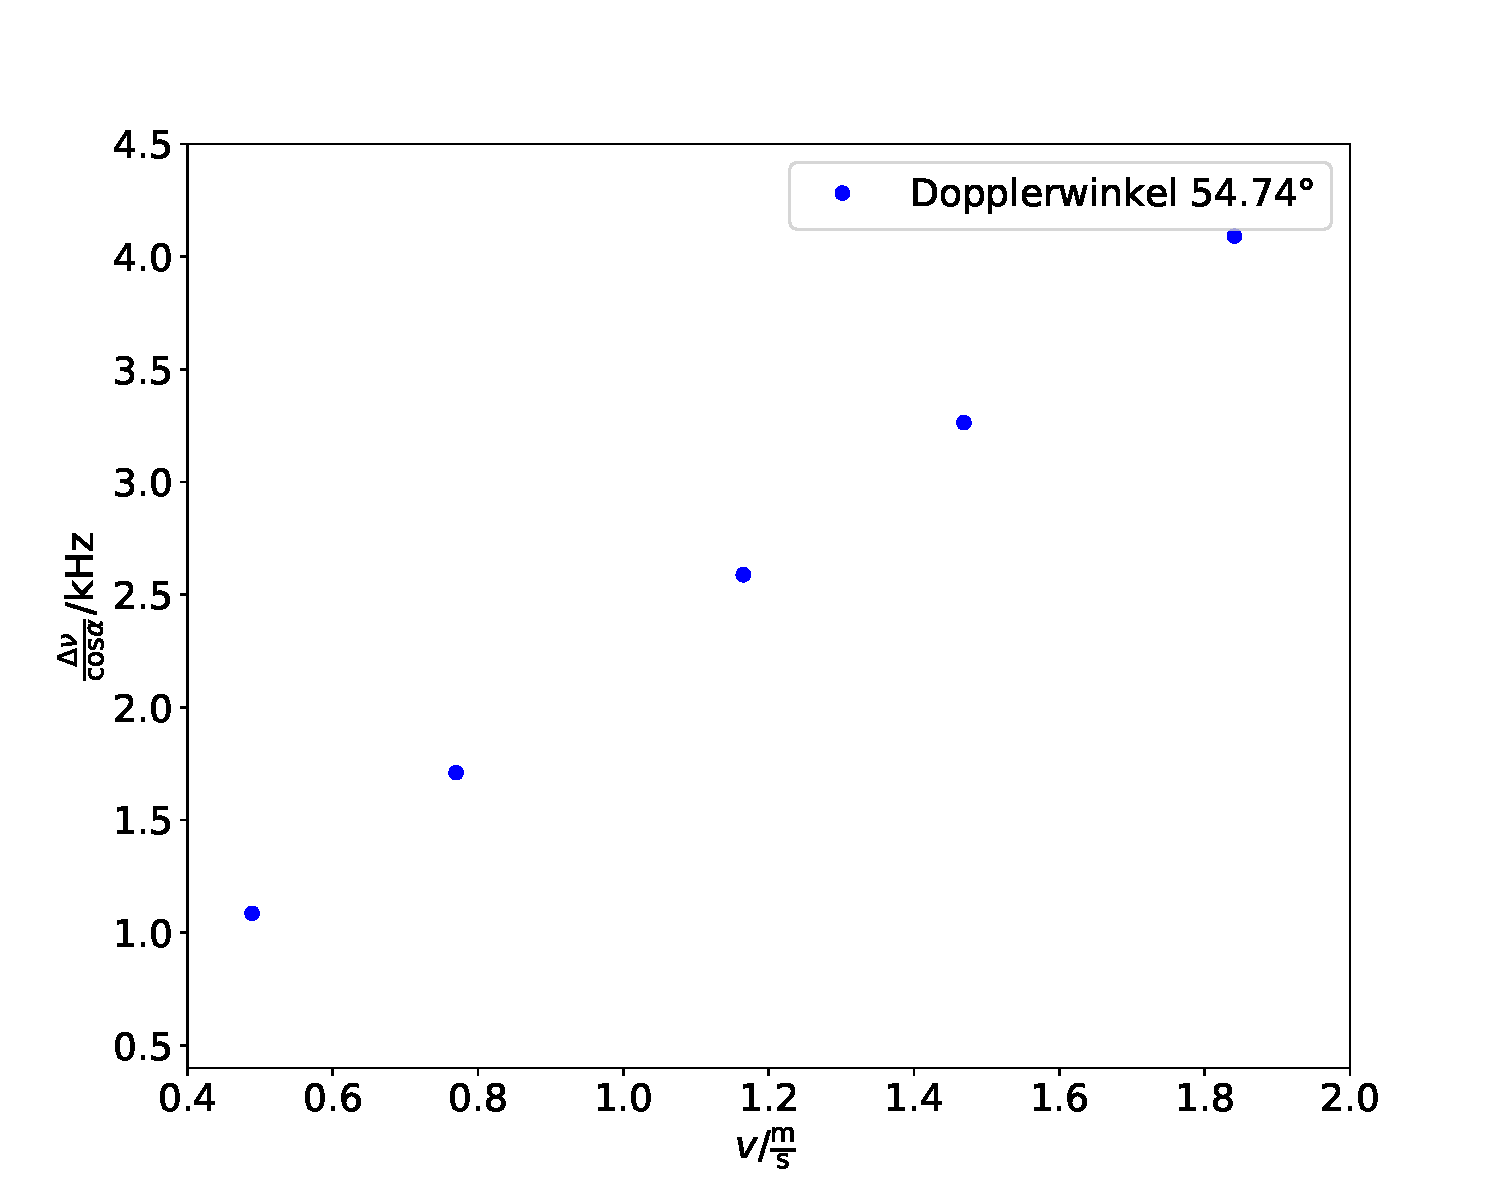
\includegraphics[width=\textwidth]{a60.pdf}
          \caption{Die Frequenzverschiebung geteilt durch den cos des Dopplerwinkels 54.74° aufgetragen gegen die Geschwindigkeit.}
          \label{fig:3}
          \qquad
      \end{subfigure}
      \begin{subtable}{0.4\textwidth}
        \centering
        \begin{tabular}{c c c}
          \toprule
          Pumpleistung / $\%$ & $\symup{\Delta} \nu$ / $\si{\hertz}$ & $v$ / \si{\meter\per\second} \\
          \midrule
          30 & -256 & 0.49 \\
          40 & -403 & 0.77 \\
          50 & -610 & 1.16 \\
          60 & -769 & 1.47 \\
          70 & -964 & 1.84 \\
          \bottomrule
        \end{tabular}
        \caption{Die Pumpleistung, die Frequenzverschiebung (aus den Messungen) und die Geschwindigkeit aus \eqref{eqn:6} berechnet für einen Einfallswinkel von 60°.}
        \label{tab:4}
        \qquad
      \end{subtable}
      \caption{Ergebisse aus Aufgabenteil 1 für den Dopplerwinkel 54.74°.}
    \end{figure}


    \subsection{Bestimmung der Streuintensität und der Momentangeschwindigkeit in
      Abhängigkeit von der Messtiefe}
      Zur Bestimmung der Momentangeschwindigkeit wird \eqref{eqn:6} genutzt mit
      $\alpha = 80.06°$ und dem gemessenen Wert für $\symup{\Delta} \nu$. Für $\nu_0$
      wird $\SI{2}{\mega\hertz}$ (vgl. Kapitel \ref{aufbau}) und für $c$
      $\SI{1800}{\meter\per\second}$ verwendet. Für die Messtiefe wird die Umrechnung
         $4 \, \symup{\mu s} = 6 \, \symup{mm}$
      verwendet. Im Folgenden sind die Ergebnisse als
      Tabelle und Diagramm aufgelistet.

      \begin{figure}
        \begin{subfigure}{0.6\textwidth}
        \centering
        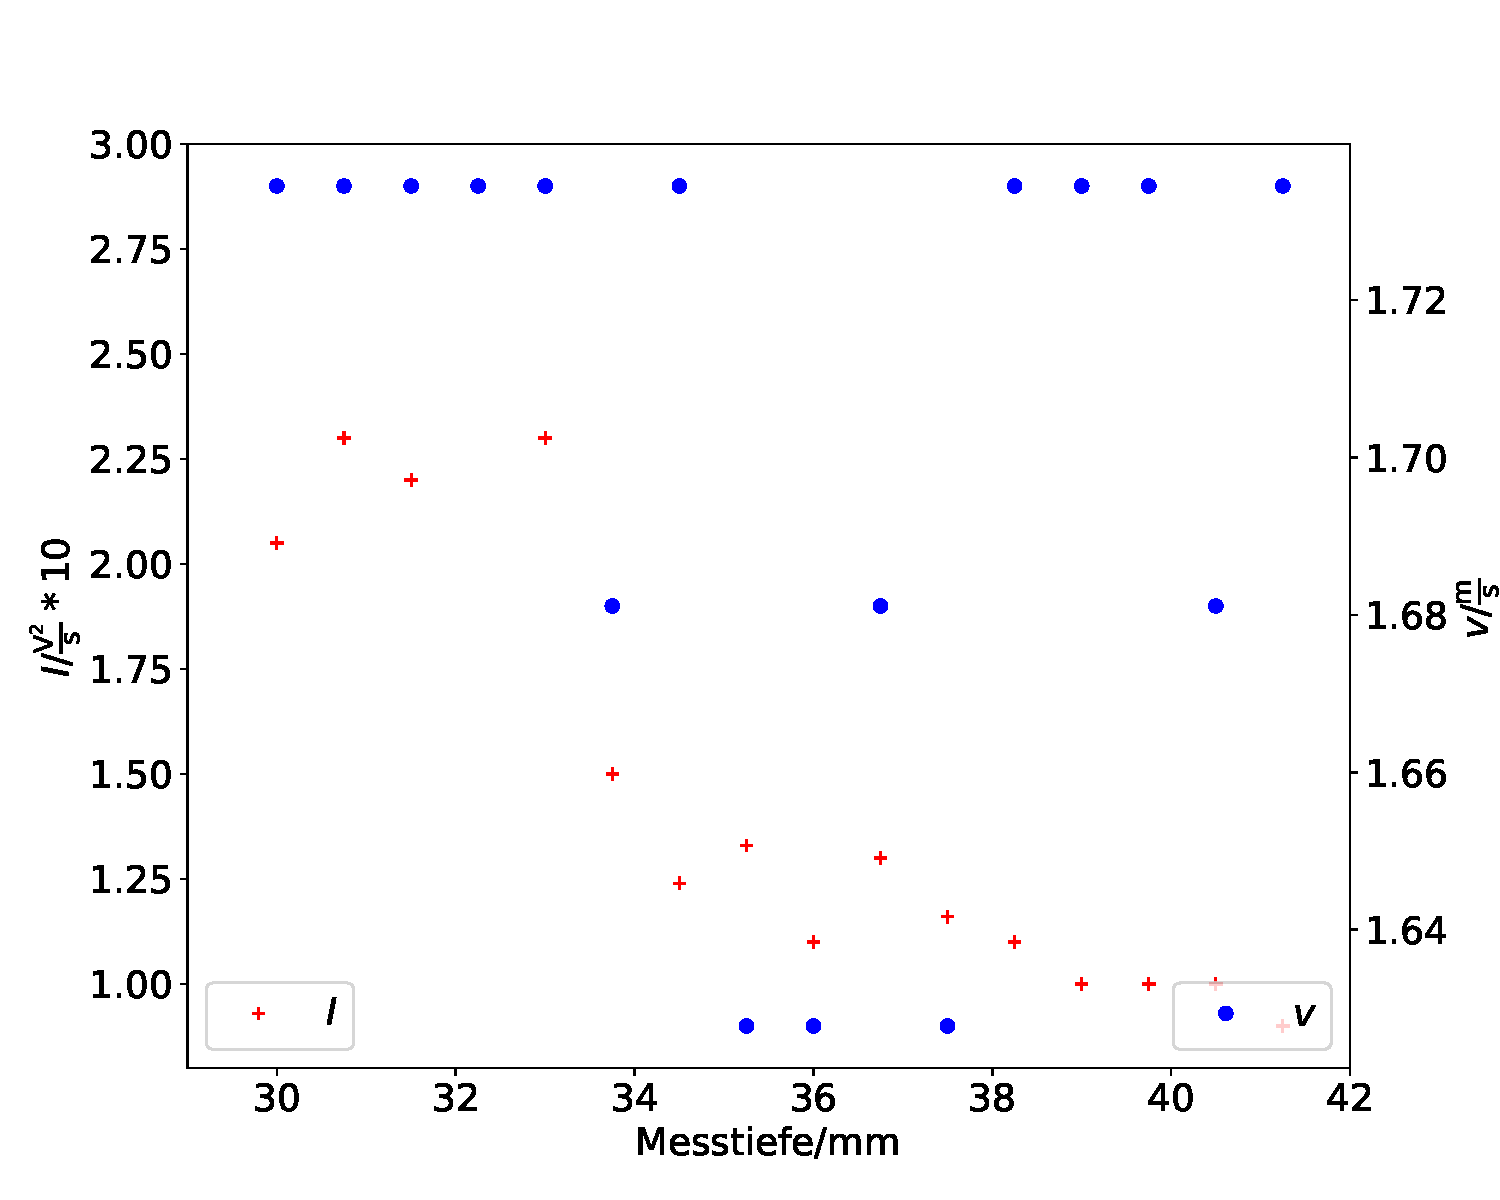
\includegraphics[width=\textwidth]{b45.pdf}
        \caption{Momentangeschwindigkeit und Streuintensität in Abhängigkeit von der Messtiefe aufgetragen.}
        \label{fig:4}
        \qquad
      \end{subfigure}
      \begin{subtable}{0.4\textwidth}
        \centering
        \begin{tabular}{c c c}
            \toprule
            Messtiefe / $\si{\meter\meter}$ & $v$ / $\si{\meter\per\second}$ & $I$ / $\si{\volt\squared\per\second} \cdot 1000$ \\
            \midrule
            30 & 1.73 & 205 \\
            30.75 &  1.73 & 230 \\
            31.5 & 1.73 & 220 \\
            32.25 & 1.73 & 290 \\
            33 & 1.73 & 230 \\
            33.75 &  1.68 & 150 \\
            34.5 & 1.73 & 124 \\
            35.25 & 1.63 & 133 \\
            36 & 1.63 & 110 \\
            36.75 & 1.68 & 130 \\
            37.5 & 1.63 & 116 \\
            38.25 & 1.73 & 110 \\
            39 & 1.73 & 100 \\
            39.75 & 1.73 & 100 \\
            40.5 & 1.68 & 100 \\
            41.25 & 1.73 & 90 \\
            \bottomrule
        \end{tabular}
        \caption{Messtiefe, Momentangeschwindigkeit $v$ aus \eqref{eqn:6} berechnet und Streuintensität $I$.}
        \label{tab:5}
        \qquad
      \end{subtable}
      \caption{Ergebnisse aus Aufgabenteil 2 für 45 $\%$ Pumpleistung.}
    \end{figure}

      \begin{figure}
        \begin{subfigure}{0.6\textwidth}
        \centering
        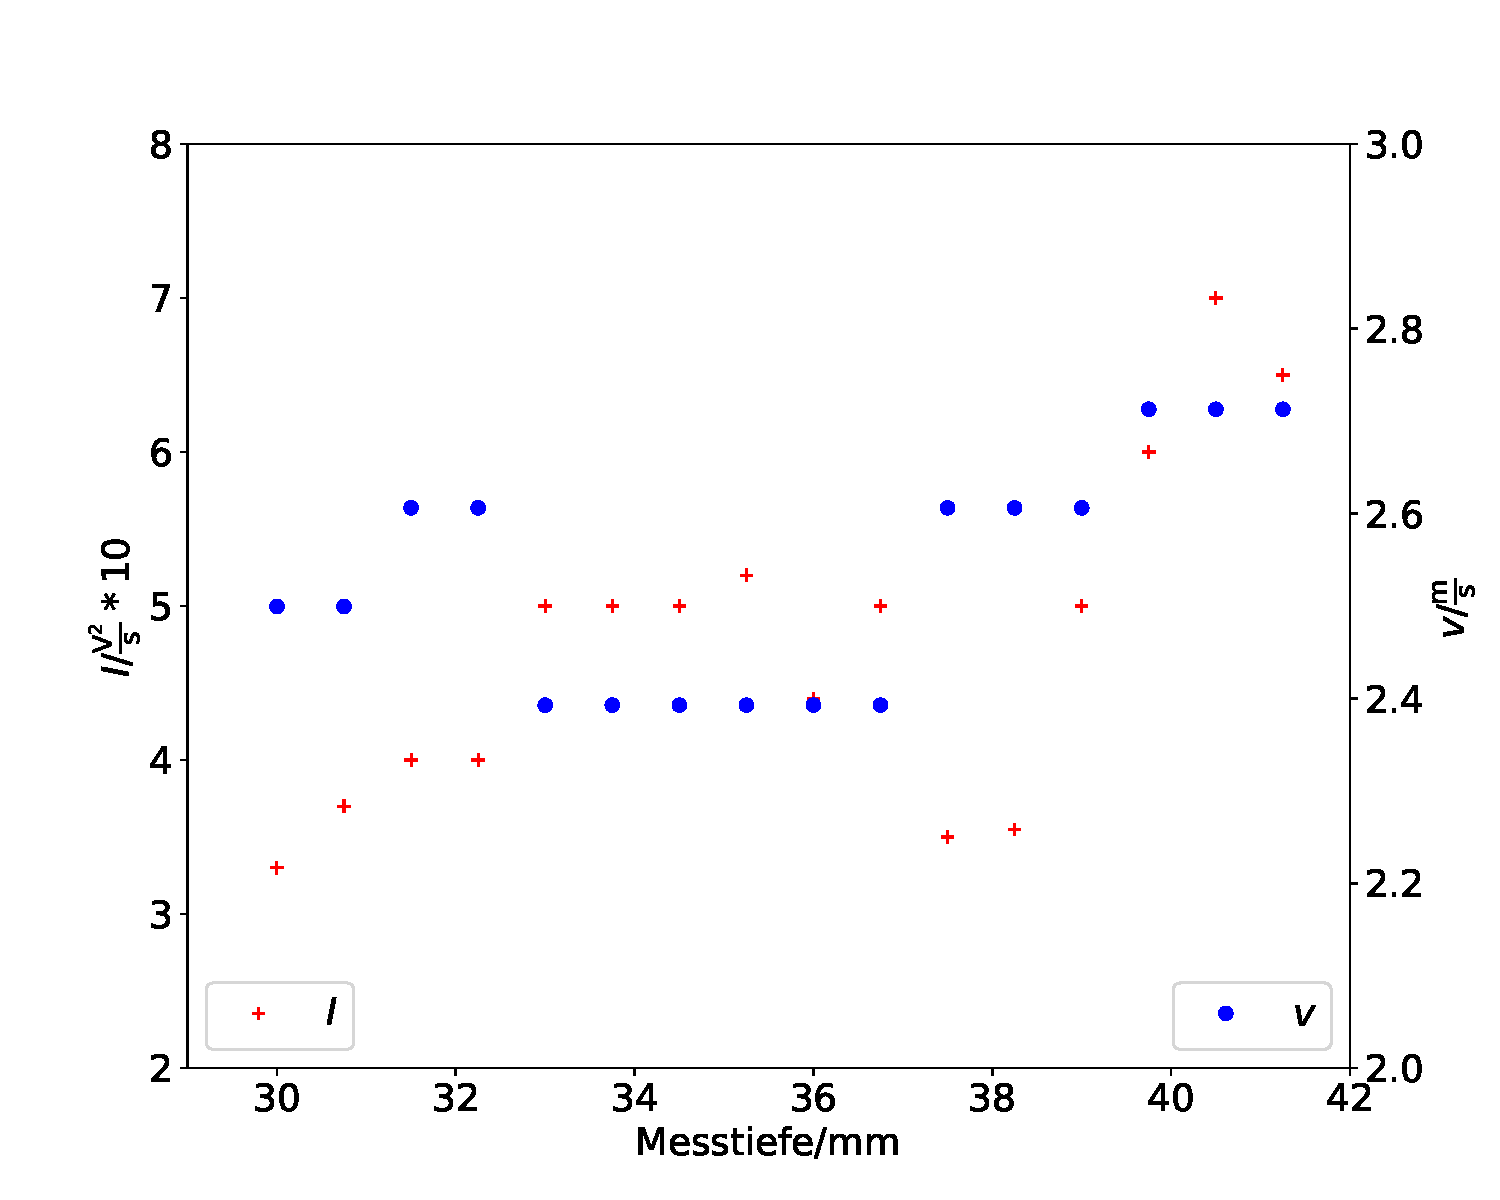
\includegraphics[width=\textwidth]{b70.pdf}
        \caption{Momentangeschwindigkeit und Streuintensität in Abhängigkeit von der Messtiefe aufgetragen.}
        \label{fig:5}
        \qquad
      \end{subfigure}
      \begin{subtable}{0.4\textwidth}
        \centering
        \begin{tabular}{c c c}
          \toprule
          Messtiefe / $\si{\meter\meter}$ & $v$ / $\si{\meter\per\second}$ & $I$ / $\si{\volt\squared\per\second} \cdot 1000$ \\
          \midrule
          30 & 2.50 & 330 \\
          30.75 & 2.50 & 370 \\
          31.5 & 2.61 & 400 \\
          32.25 & 2.61 & 400 \\
          33 & 2.40 & 500 \\
          33.75 & 2.40 & 500 \\
          34.5 & 2.40 & 500 \\
          35.25 & 2.40 & 520 \\
          36 & 2.40 & 440 \\
          36.75 & 2.40 & 500 \\
          37.5 & 2.61 & 350 \\
          38.25 & 2.61 & 355 \\
          39 & 2.61 & 500 \\
          39.75 & 2.71 & 600 \\
          40.5 & 2.71 & 700 \\
          41.25 & 2.71 & 650 \\
          \bottomrule
        \end{tabular}
        \caption{Messtiefe, Momentangeschwindigkeit $v$ aus \eqref{eqn:6} berechnet und Streuintensität $I$.}
        \label{tab:6}
        \qquad
      \end{subtable}
      \caption{Ergebnisse aus Aufgabenteil 2 für 70 $\%$ Pumpleistung.}
    \end{figure}


\section{Diskussion}
Aus den Diagrammen \ref{fig:1} bis \ref{fig:3} folgt, dass ein linearer Zusammenhang
zwischen dem Verhältnis aus Frequenzverschiebung und dem Cosinus des Dopplerwinkels und
der Strömungsgeschwindigkeit vorliegt. Außerdem stimmen die Strömungsgeschwindigkeiten bei
den Einstrahlwinkeln 30° und 60° mit einer maximale Abweichung von \SI{0.11}{\meter\per\second}
gut überein. Lediglich die Werte für den Einstrahlwinkel von 15° weichen stark ab. Hier liegt die
maximale Abweichung bei \SI{1.42}{\meter\per\second} im Vergleich zu der Messung bei 30°
bzw. bei \SI{1.31}{\meter\per\second} unter einem Winkel von 60°. Eine mögliche
Erklärung ist, dass die Messung für diesen Winkel als erstes vorgenommen wurde, sodass
noch Lufteinschlüsse in der Apperatur vorhanden waren, die nach einiger Pumpenlaufzeit
zum Luftauslass transportiert wurden. Desweiteren konnte eine gute Fixierung des Doppler-Prismas
auf dem Strömungsrohr anfangs nicht gewährleistet werden. Die Messung bei 15° sollte
daher wiederholt werden.\\
\\
%Die Messreihe zur Bestimmung des Strömungsprofils ermöglicht hingegen keine sinnvolle
%Auswertung. Die Momentangeschwindigkeit ändert sich durch den Rohrquerschnitt nicht
%signifikant.
Aus Abbildung \ref{fig:4} lässt sich erkennen, dass die Geschwindigkeit zum Rand des Rohrs hin
konstant ist, während sie in der Mitte des Rohrs ein Minimum hat, was dem Modell widerspricht.
Ähnliches gilt für Abbildung \ref{fig:5}, wobei bei 70\% Pumpleistung die Strömungsgeschwindigkeit zum Rand hin weniger
konstant ist, aber weiterhin ein Minimum zur Rohrmitte hin aufweist.
Die Streuintensität schwankt ohne erkennbares Muster über den gesamten
Querschnitt. Aufgrund dieser Ergebnisse sind systematische Messfehler zu vermuten,
welche die Messung derart beeinflusst haben, dass keine Aussagen mehr möglich sind.
Möglich ist hier eine Blockade des Flüssigkeitsstroms durch Knicke in den nicht
starren Kurvenstücken. Dieser zweite Versuchsteil kann daher in der jetzigen Form keine Ergebnisse
liefern und sollte zwecks Prüfung wiederholt werden.\\
\\
Außerdem lässt sich sagen, dass sich das Ablesen der vom Computer angezeigten Werte bei beiden Versuchsteilen
als schwierig gestaltet hat, da sich die Werte teilweise im Sekundenintervall änderten.
Dadurch sind systematische Fehler nicht auszuschließen. Abschließend lässt sich feststellen,
dass der erste Teil des Versuchs gute Ergebnisse geliefert hat, während der zweite Teil
aufgrund der aufgenommenen Messwerte nicht zufriedenstellend ausgewertet werden kann.
\newpage
\nocite{*}
\printbibliography
